% \pagebreak[4]
% \hspace*{1cm}
% \pagebreak[4]
% \hspace*{1cm}
% \pagebreak[4]

\chapter{My First Chapter But Note The Numbering ...}
\ifpdf
    \graphicspath{{Chapter1/Chapter1Figs/PNG/}{Chapter1/Chapter1Figs/PDF/}{Chapter1/Chapter1Figs/}}
\else
    \graphicspath{{Chapter1/Chapter1Figs/EPS/}{Chapter1/Chapter1Figs/}}
\fi
\markboth{\MakeUppercase{\thechapter. My First Chapter }}{\thechapter. My First Chapter}

\section{First Paragraph}

And now I begin my first chapter here ...

Here is an equation\footnote{the notation is explained in the nomenclature section :-)}:
\begin{eqnarray}
CIF: \hspace*{5mm}F_0^j(a) &=& \frac{1}{2\pi \iota} \oint_{\gamma} \frac{F_0^j(z)}{z - a} dz
\end{eqnarray}
\nomenclature[zcif]{$CIF$}{Cauchy's Integral Formula}                                % first letter Z is for Acronyms 
\nomenclature[aF]{$F$}{complex function}                                                   % first letter A is for Roman symbols
\nomenclature[gp]{$\pi$}{ $\simeq 3.14\ldots$}                                             % first letter G is for Greek Symbols
\nomenclature[gi]{$\iota$}{unit imaginary number $\sqrt{-1}$}                      % first letter G is for Greek Symbols
\nomenclature[gg]{$\gamma$}{a simply closed curve on a complex plane}  % first letter G is for Greek Symbols
\nomenclature[xi]{$\oint_\gamma$}{integration around a curve $\gamma$} % first letter X is for Other Symbols
\nomenclature[rj]{$j$}{superscript index}                                                       % first letter R is for superscripts
\nomenclature[s0]{$0$}{subscript index}                                                        % first letter S is for subscripts

\section{Second Paragraph}
and here I write more ...\cite{texbook}

\subsection{Mendeley}

Mendeley is not necessary for \LaTeX.  Mendeley is a standalone referencing management system that can be integrated to Microsoft Word or with \LaTeX.  The Mendeley application will manage your references in a manner similar to EndNote.  The major advantage of Mendeley is that it will also manage your downloaded .pdf files.  For more details of Mendeley and its functionality please go to \href{http://www.mendeley.com/}{www.mendeley.com} 





\subsection{MiKTeX}

The MiKTeX distribution contains the source files and executables for \LaTeX  to work.  The MiKTex distribution comes is available  from \href{http://miktex.org/}{miktex.org}  Please note that a completed installation will consume approx 2.0 Gig of hard disk space.  As the system is based on 'packages' you can elect to download and install packages as they are required.  This will substantially reduce the hard disk requirement; however it can pose problems when internet connectivity is lost.  My preferred option is to install the full distribution.  


\subsection{TeXnicCenter}

In order to use \LaTeX you will need a text editor.  There are numerous editors available for free download.  To date I have found TeXnicCenter to be the most flexible.  TeXnicCenter is available from  \href{http://www.texniccenter.org/}{www.texniccenter.org} 






\subsection{Referencing and Citation}
... and some more ...

Now I would like to cite the following: \cite{latex} and \cite{texbook}
and \cite{Rud73}.

Referencing or citation can be achieved in a number of formats.  The standard is the \verb|\cite| command which will display as above.  Alternatives are \verb|\citet| and   \verb|\citep|.  The \verb|\citet| command produces \citet{KR83} whereas the \verb|\citep| command produces \citep{latex}.  More information is available from the  \href{http://merkel.zoneo.net/Latex/natbib.php}{Natbib Reference Sheet by Ross Moore}

\subsection{Including Figures and Pictures}


I would also like to include a picture ...

\begin{figure}[!htbp]
  \begin{center}
    \leavevmode
    \ifpdf
      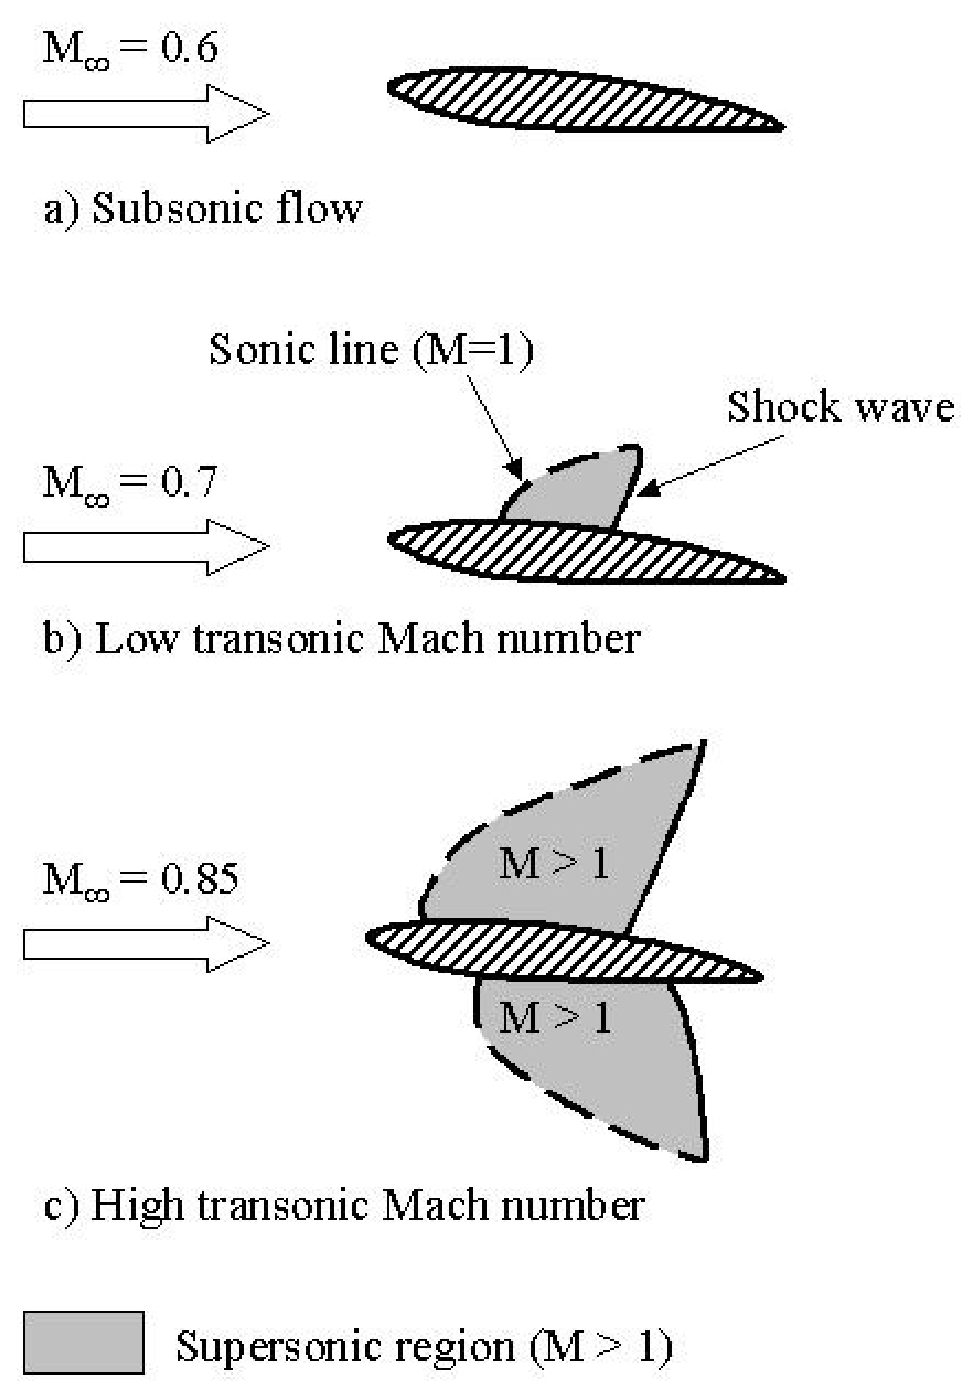
\includegraphics[height=6in]{aflow}
    \else
      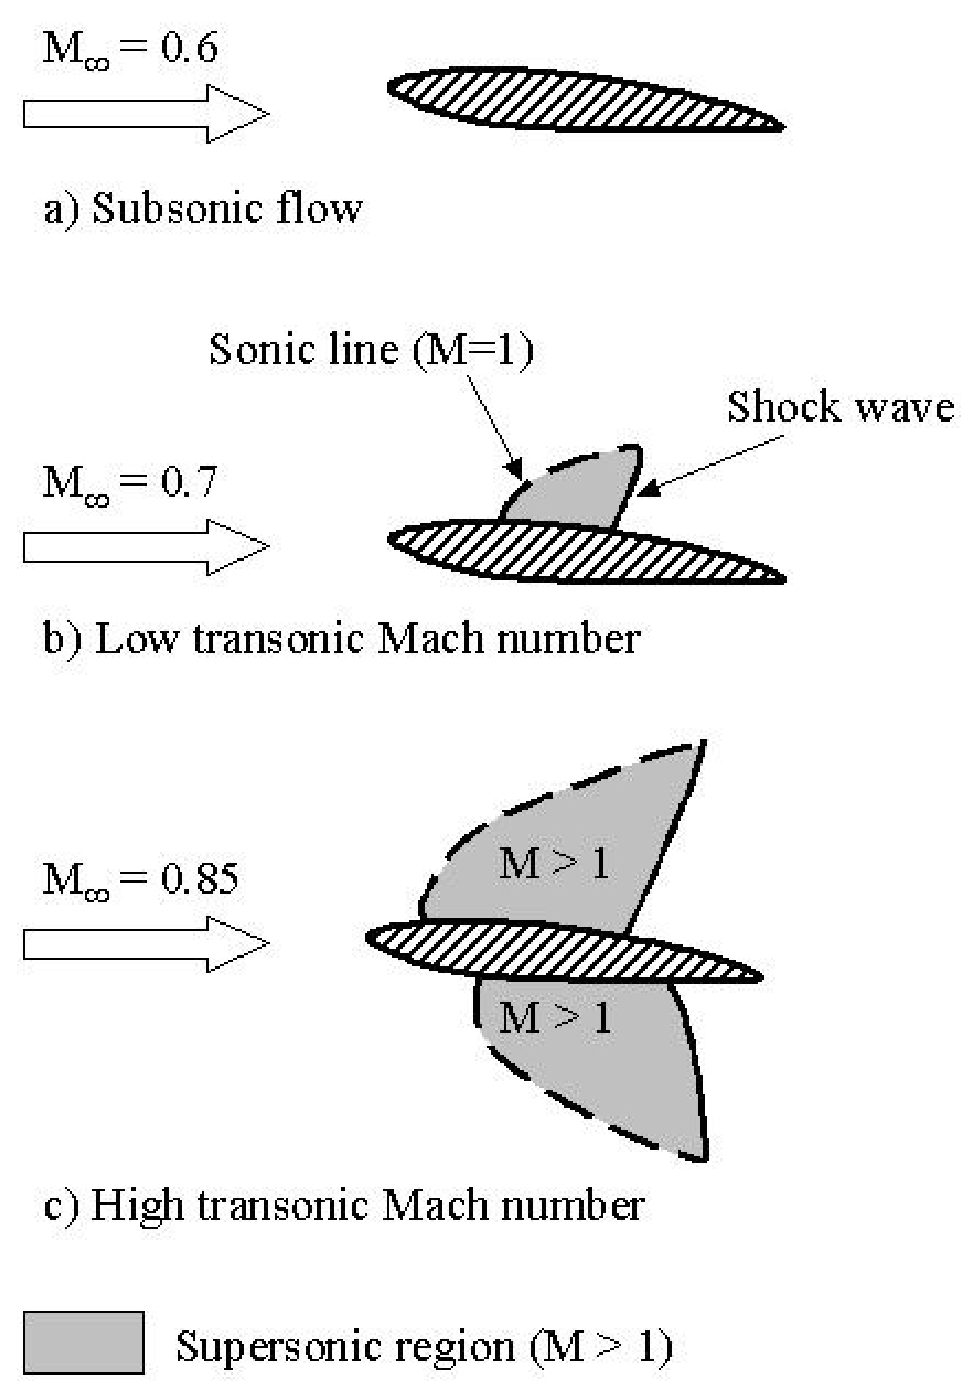
\includegraphics[bb = 92 86 545 742, height=6in]{aflow}
    \fi
    \caption{Airfoil Picture}
    \label{FigAir}
  \end{center}
\end{figure}

% above code has been macro-fied in Classes/MacroFile.tex file
%\InsertFig{\IncludeGraphicsH{aflow}{6in}{92 86 545 742}}{Airfoil Picture}{FigAir}

So as we have now labelled it we can reference it, like so (\ref{FigAir}) and it
is on Page \pageref{FigAir}. And as we can see, it is a very nice picture and we
can talk about it all we want and when we are tired we can move on to the next
chapter ...

I would also like to add an extra bookmark in acroread like so ...
\ifpdf
  \pdfbookmark[2]{bookmark text is here}{And this is what I want bookmarked}
\fi
% ------------------------------------------------------------------------


%%% Local Variables: 
%%% mode: latex
%%% TeX-master: "../thesis"
%%% End: 
